\documentclass[10pt,a4paper,ngerman]{scrartcl}
\usepackage[utf8]{inputenc}
\usepackage[ngerman]{babel}
\usepackage[T1]{fontenc}
\usepackage{amsmath}
\usepackage{amsfonts}
\usepackage{amssymb}
\usepackage{makeidx}
\usepackage{graphicx}
\usepackage{epstopdf}
\usepackage[onehalfspacing]{setspace}
\usepackage{array}
\usepackage{upgreek}
\usepackage{float}
\usepackage{csquotes}
\usepackage{chemformula}
\usepackage{chemgreek}
\usepackage{chemmacros}
\chemsetup{modules=all}
\usepackage{tikz}
\usepackage{siunitx}
\sisetup{locale = DE,per-mode = symbol}
\usepackage{esvect}
\usepackage{geometry}
\usepackage{graphicx}
\usepackage{subcaption}
\usepackage{pdfpages}
\usepackage[font=small]{caption}
%\usepackage[version=4]{mhchem}
\usepackage[backend=biber, style=chem-angew]{biblatex}
\addbibresource{CoPo.bib}
\usepackage{tabularx, booktabs, multirow}
\usepackage[pdfborder={0 0 0}]{hyperref}
\usepackage{scrlayer-scrpage}%Header für die KOMA-script -Klasse
%\usepackage{hyperref}
\usepackage{pgfplots}
\usepackage{textgreek}


\newcommand{\tildenu}{{\fontencoding{LGR}\selectfont\accperispomeni\textnu}}
\captionsetup{format=plain}
\chemsetup[phases]{pos=sub}
\chemsetup[redox]{pos=top}
\chemsetup[redox]{align=center}
%\chemsetup[redox]{explicit-sign=true}
%\chemsetup[redox]{roman=false}
\newcommand{\celsius}{^{\circ}\mathrm{C}}
\parindent0pt
\sloppy
\DeclareChemPhase{\s}{s}
\DeclareChemPhase{\l}{l}
\DeclareChemPhase{\g}{g}
\renewcaptionname{ngerman}{\figurename}{Abb.}
\renewcaptionname{ngerman}{\tablename}{Tab.}
\geometry{bottom=100pt} \geometry{top=80pt}
\newcommand{\m}{\mathrm{m}}
\newcommand{\K}{\mathrm{K}}
\newcommand{\J}{\mathrm{J}}
\newcommand{\gr}{\mathrm{g}}
\newcommand{\kg}{\mathrm{kg}}
\newcommand{\mol}{\mathrm{mol}}
\newcommand{\Pa}{\mathrm{Pa}}
\newcommand{\ad}{\mathrm{ad}}
\newcommand{\de}{\mathrm{de}}
\newcommand{\gmol}{\mathrm{\frac{g}{mol}}}
\newcommand{\JKmol}{\mathrm{\frac{J}{K \cdot mol}}}
\newcommand{\kgmss}{\mathrm{\frac{kg}{m \cdot s^2}}}
\newcommand{\loge}{\mathrm{ln}}


\begin{document}
\begin{titlepage}
	\vspace*{2,5cm}
	\begin{center}
		\begin{LARGE}
			\textbf{Polymer Chemie}\\
			\textbf{Radikalische (Co)Polymerisation}\\
		\end{LARGE}
		\vspace{1cm}
		\textbf{Universität Stuttgart}\\
		\vspace*{1,5cm}
		\begin{tabular}{lp{7,5cm}l}
			Author 1:     &Laurens Viehoff\\
            Author 2:     &Felix Roth\\   
			E-Mail 1:      &st183688@stud.uni-stuttgart.de\\
            E-Mail 2:      &st188157@stud.uni-stuttgart.de  \\
			Student-ID 1: & 3676761   \\ 
            Student-ID 2: & 3711192 \\ \\
			Assistentin:  & Florian Rausch  \\ \\ 
		\end{tabular}
	\end{center}

    
\end{titlepage}
\thispagestyle{empty}
\renewcommand{\thepage}{\arabic{page}}
\newpage
\tableofcontents
\setcounter{page}{1}
\renewcommand{\thepage}{\arabic{page}}
\newpage


\section{Theorie}

	Im Allgemeinen lässt sich die radikalische Polymerisation in drei Teilschritte unterteilen.
	Der erste Schritt ist der Kettenstart, hierbei wird mittels eines Radikalstarters (im Falle des Versuchs AIBN), durch thermischen Zerfall ein Radikal gebildet (\ref{Kettenstart}).

	
		\begin{figure}[H]
			\centering
			
\includegraphics[scale = 0.25]{Bilder/Initiierung.png}
			\caption{Die Abbildung zeigt den thermischen Zerfall von AIBN. }
			\label{Kettenstart}
		\end{figure}

	Dieses gebildete Radikal greift radikalisch an dem vinylischen Kohlenstoff an.
	Dabei wird die $\pi$-Bindung geöffnet und es bildet sich eine neue $\sigma$-Bindung.
	Dabei entsteht das Radikal an der benzylischen Stelle.
	Wichtig ist jedoch, dass nicht alle Radikale des Initiators an der Polymerisation beteiligt sind.
	Dafür lässt sich der Radikal-Ausbeute-Faktor $f$ bestimmen.
		
		\begin{equation}
			f = \frac{\sum \text{kettenstart}R^*}{\sum \text{gebildete}R^*}
			\label{Cage-Effekt}
		\end{equation}
	
	Dabei sind R* die jeweiligen Radikale die einerseits durch thermischen Zerfall gebildet wurden,
	und die gebildeten Radikalen entsprechen den gebildeten Starter und Monomer Kombinationen.
	Der zweite Schritt besteht aus dem Kettenwachstum. Hierbei wird die Polymerkette mittels weiterem Monomer gebildet.

		\begin{figure}[H]
			\centering
			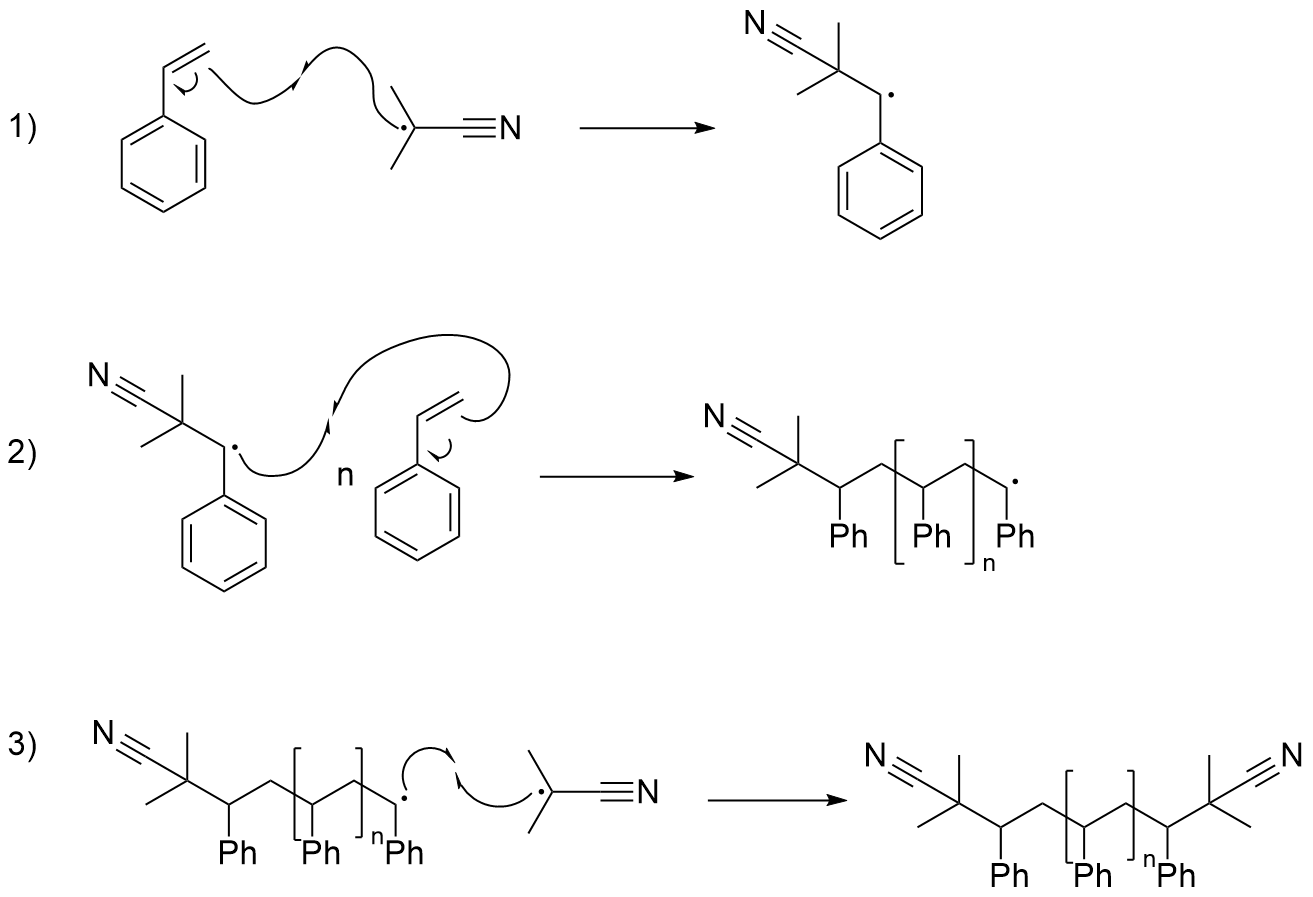
\includegraphics[scale = 0.4]{Bilder/RadikalKomplett.png}
			\caption{Die Abbildung zeigt die radikalische Polymerisation mit Start, Wachstum und Abbruch. 
			Als Abbruch wurde hier eine Rekombination als Beispiel gewählt.}
			\label{Radikalisch_Komplett}
		\end{figure}

	Für diesen Schritt lässt sich ein Geschwindigkeitsgesetzt aufstellen, welches die Wachstumsgeschwindigkeit $v_w$ und die Geschwindigkeitskonstante $k_w$ berücksichtigen.
	
		\begin{equation}
			v_w = k_w [p^*][M]
			\label{Zeitgesetzt}
		\end{equation}

	Der letzte und dritte Schritt ist der Abbruchsschritt. Bei diesem gibt es zwei Möglichkeiten eines Abbruchs.
	Der erste wäre die Rekombination auch in Abb. \ref{Radikalisch_Komplett} gezeigt. Hierbei reagieren zwei Radikale miteinander und bilden eine Bindung aus. 
	Das reaktive Radikal geht somit verloren.\\ 
	Die andere Variante wäre eine Disproportionierung. Hierbei findet eine radikalische Bindung zwischen einem Monomer und dem $\alpha$-Wasserstoff statt. 
	Dabei findet zusätzlich eine Rekombination zu einer Doppelbindung statt. 
	
	
	%Vielleicht Gleichung


	Desweiteren kann der Umsatz in abhängigkeit zu dem Polymerisationsgrad aufgetragen werden, wordurch folgender Graph entsteht. \supercite{polyskript}

		\begin{figure}[H]
			\centering
			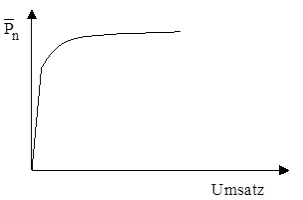
\includegraphics[scale = 0.7]{Bilder/GraphPG.png}
			\caption{Die Abbildung beschreibt die Abhängigkeit des Polymerisationsgrad vom Umsatz. \supercite{polyskript}}
			\label{GraphPG}
		\end{figure}


\subsection{Kinetik der radikalischen Polymerisation}
	Für diese Kinetik spielt auch das sogenannte Wurzel-I-Gesetz eine große Rolle. 
		
	Um dieses Aufstellen zu können wird unteranderem von sechs Annahmen ausgegangen.\\
	
	Die erste ist, dass vorhandensein einer irreversieblen Reaktion.\\
	
	Die zweite ist, dass die Initiatorradikal-konzentration stationär ist. 
	Was soviel bedeutet wie, gleich viele Radikale werden durch Zerfall des Initiators gebildet wie verbraucht werden.\\

	Die dritte Beschreibt, dass die Initiatorkonzentration während der Polymerisation konstant bleibt.\\

	Die vierte beschreibt im großen und ganzen, dass die Bruttoreaktionsgeschwindigkeit $v_\text{Br}$ und die Wachstumsreaktionsgeschwindigkeit $v_w$ gleich sind woduch folgt:

		\begin{equation}
			v_\text{Br} \approx v_w = k_w [P^*][M]
		\end{equation}

	Die fünfte, ist das ausgehen von einem Abbruch welcher lediglich durch gegenseitige Desaktivierung der Polymere erfolgt.\\

	Die sechste und letzte ist ähnlich wie die zweite nur das davon ausgegangen wird, dass die Polymerradikal-konzentration stationär ist.\\

	Das Wurzel-I-Gesetz definiert die Bruttoreaktionsgeschwindigkeit und ist in Gleichung \ref{WurzelI} beschrieben

		\begin{equation}
			v_\text{Br} = k_w \sqrt{\frac{2k_z f}{k_{ab}}}\sqrt{[I]}[M]
			\label{WurzelI}
		\end{equation}

	Um diese Geschwindigkeiten zu bestimmen werden Eigenschaften wie Volumen der Polymerlösung, 
	Abnahme der Monomerkonzentration oder die Zunahme der Polymermenge verwendet. 
	Desweiteren ist die Bruttogeschwindigkeit abhängig von der Konzentration der Edukte.\\

	Allgemein wird um die Güte einer Polymerisation zu bestimmen der zahlenmittlere Polymerisationsgrad bestimmt. 
	Dieser wird in zwei unterschiedlichen Formeln beschrieben wobei Formel (\ref{Pn1}) den Polymerisationsgrad bei Abbruch durch Kombination beschreibt, 
	und Formel (\ref{Pn2}) den Polymerisationsgrad bei Kettenabruch durch Disproportionierung beschreibt.

		\begin{equation}
			\bar{P_n} = 2v\\
			\label{Pn1}
		\end{equation}

		\begin{equation}
			\bar{P_n} = v
			\label{Pn2}
		\end{equation}
		
	Dies lässt sich auch für Kettenübertragungen betrachten wobei hier die Kettenlänge $v$ durch $v'$ ausgetauscht wird. 
	Dieser wird auch als Polymerkette bezeichnet und beschreibt alle Monomere die im Wachstum polymerisiert wurden. 
	Wichtig dabei ist auch, dass die für die Disproportionierung sowie für die dur eine Übretragung abgebrochenen Reaktion die Formel (\ref{PnV'1}) gilt.
	Aber für Reaktionen die durch Kombination abgebrochen wurden Formel (\ref{PnV'2})

		\begin{equation}
			\bar{P_n} = v'
			\label{PnV'1}
		\end{equation}
		\begin{equation}
			\bar{P_n} = 2v'
			\label{PnV'2}
		\end{equation}

	E. Trommsdorff entdeckte den nach ihm benannten Norrish-Trommsdorff-Effekt, welcher einen starken Anstieg der Geschwindigkeit bei hohen Umsätzen beschreibt. 
	Er erklärte dies durch einen Anstieg der Viskosität bei kontinuierlicher Polymerisation, 
	da die Ketten immer länger werden und ihre Bewegung eingeschränkt wird. Durch die Einschränkung der Bewegung können die Kettenradikale nur schwer rekombinieren 
	und die radikale bleiben erhalten. Da das Monomer aber noch eine hohe Beweglichkeit besitzt, diffundiert dieses durch die Lösung und wird durch eine hohe 
	Radikalkonzentration leicht polymerisiert. Bei fast 100 \% Umsatz lässt dann die Geschwindigkeit nach, da die Monomerkonzentration stark gegen null geht. \supercite{polyskript}

		\begin{figure}[H]
			\centering
			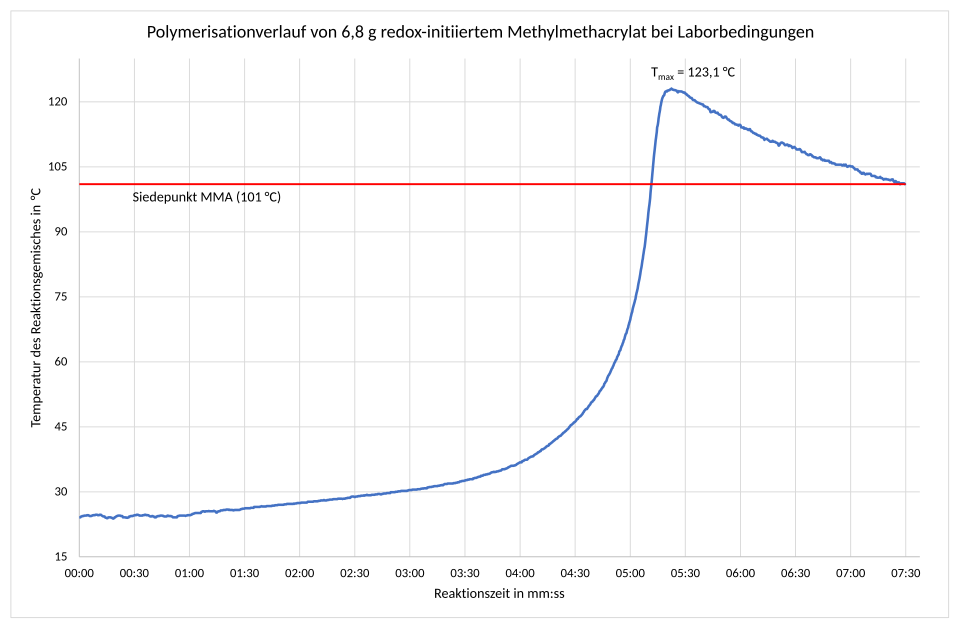
\includegraphics[scale = 0.3]{Bilder/Norrish-Trompsdorff.png}
			\caption{Die Abbildung zeigt den Norrish-Trommsdorff-Effekt Graphish dargestellt.\supercite{noauthor_dateipolymerisationsverlauf_2018}}
			\label{NTE}
		\end{figure}

	
\subsection{Kinetik der radikalischen Copolymerisation}

	Auch bei der Copolymerisation wird mit Annahmen gearbeitet. Hier sind es jedoch nur fünf welche zum Aufstellen der Copolymerisationsgleichung benötigt werden.\\

	Die erste ist identisch zu der zuvor genannten ersten Annahme, dass alle Reaktionen irreversiebel sind.\\

	Die zweite beschreibt, dass die Bruttokonzentrationen der Monomere gleich der Konzentrationen am Reaktionsort sein muss.\\

	Die dritte ist das Vernachlässigen des Monomerverbrauchs am Start, Abbruch und Übertragung da ein sehr hoher Polymerisationsgrad vorhanden ist.\\

	Die vierte ist das Vernachlässigen der Reaktivität des zuvor eingebauten Monomers.\\

	Die letzte ist die Annahme, das für die Kinetik das Bodenstein'sche Quasistationaritätsprinzip gilt.\\

	Mit diesen Annahmen kann das Ziel einer Aussage zum Einbauverhältnis verfolgt werden. 
	Dafür werden folgende Reaktionsgleichungen mit der jeweiligen Reaktionsgleichungen:

		\begin{figure}[H]
			\centering
			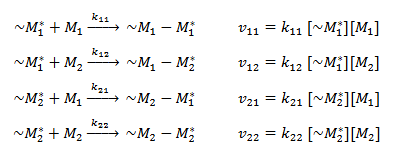
\includegraphics[scale = 0.75]{Bilder/RGL.png}
			\caption{Die Abbildung zeigt die Reaktionsgleichungen aller möglichen Wachstumsreaktionen. \supercite{polyskript}}
			\label{RGL_wachstum}
		\end{figure}

	Durch Umformen und einsetzen folgt aus diesen Reaktionsgleichungen die Copolymerisationsgleichung.

		\begin{equation}
			\frac{m_1}{m_2} = \frac{[M_1]}{[M_2]}\cdot \frac{r_1[M_1]+[M_2]}{r_2[M_2]+[M_1]}
		\end{equation}

	Darin sind $r_i$ die Copolymerisationskonstanten, welche als $\frac{k_{ii}}{k_{ij}}=r_i$ definiert sind.
	Unteranderem besdchreibt $m$ den jeweiligen Anteil des Monomers im Copolymer. Und $[M]$ ist die jeweilige Monomer konzentration.\\
	Experimentell werden diese Parameter über Spektroskopie wie NMR oder IR bestimmt, können aber auch durch Elementaranalyse bestimmt werden.\\

	Durch Umformen der zuvor genannten Gleichung kann eine lineare Beziehung gezeigt werden und folgende Funktion aufgestellt werden:

		\begin{equation}
			r_1 = r_2 \frac{m_1[M_2]^2}{m_2[M_1]^2} + \frac{[M_2]}{[M_1]}\cdot \left(\frac{m_1}{m_2}-1\right)
			\label{CoPO-r1r2}
		\end{equation}

	Daraus gehen Steigung sowie der Ordinatenabschnitt heraus und es lässt sich eine Gerade zeichnen. 
	So lässt sich die Copolymerisationsparameter durch den Schnittpunkt der unterschiedlichen Geraden ermitteln.
	Da dies jedoch nicht immer der Fall ist, wird ein arithmetisches Mittel gebildet (auch in Abb. \ref{GraphMittel} zu sehen).

		\begin{figure}[H]
			\centering
			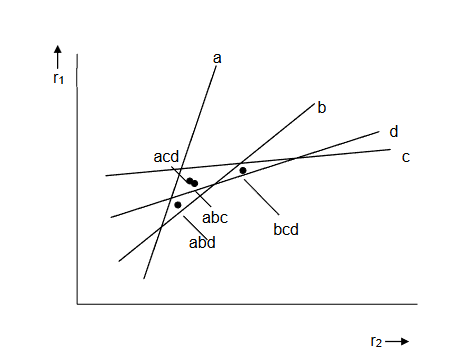
\includegraphics[scale = 0.75]{Bilder/GraphMittel.png}
			\caption{Graphische Copolysmerisationsparameterbestimmung.\supercite{polyskript}}
			\label{GraphMittel}
		\end{figure}

	Dies ist die Methode nach Mayo und Lewis. Eine Andere Methode, welche auch eine graphische Bestimmung verwendet, ist die nach Fineman und Ross.
	Dabei die Copolymerisationsgleichung so umgeformt, das beide $r$ die Steigung und den Ordinatenabschnitt angeben.

		\begin{equation}
			\frac{[M_1]}{[M_2]}\cdot \left( 1- \frac{m_2}{m_1}\right) = r_1 \cdot \frac{[M_1]^2\cdot m_2}{[M_2]^2 \cdot m_1} - r_2
			\label{FinemanRoss}
		\end{equation}

	Dabei werden die ergebenen Punkte geplottet und anschließend über eine Ausgleichsgerade der Achsenabschnitt und die Steigung bestimmt.\\


	Diese Copolymerisationsparameter können generell durch unterschiedliche Dinge beeinflusst werden. 
	So kann die generelle Konstitution der Monomere, Resonanzstabilisierung der Monomers sowie des Polymerradikals, 
	das Lösemittel, die Sterik und die Doppelbindungspolarität eine Rolle spielen. \supercite{polyskript}


\section{Durchführung}

		Alle Versuche wurden unter Schlenk-Bedingungen durchgeführt, und es wurde auf eine Argon-Athmosphäre und wasserfreie Umgebung geachtet.\\

	\subsection{Teil 1}

		In kleinen Schraub-Septum-Gläschen wurden drei unterschiedliche AIBN-Lösungen vorgelegt. 
		In das erste wird eine $0,15\cdot 10^{-2}\text{M}$, in das zweite eine $0,6\cdot 10^{-2}\text{M}$ und in das letzte eine $1,5\cdot 10^{-2}\text{M}$ Lösung gegeben. 
		Hierzu wird jeweils Styrol $\SI{10}{ml}$ zugegeben, und für 15 min mit Stickstoff entgast. 
		Es wird ein Heitzblock auf 60°C vorgeheitzt und die Lösungen werden für 2 Stunden gerührt.
		Die Lösungen werden anschließend langsam in kaltes Methanol gegeben und das Polymer wird filtriert.
		Das flitrierte Produkt wurde im Vakuumtrockenschrank bei 60°C getrocknet.

	\subsection{Teil 2}

		In fünf Schraub-Septum-Gläschen werden Ansätze mit einer 0,5 mol\%-AIBN Lösung präpariert:

		\begin{table}[htbp]
			\centering
			\caption{Mischungsverhältnisse der beiden Monomere.}
			\label{mischungsverhaeltnisse}
			\begin{tabular}{c|c|c}
					Gläßchen & \textbf{Styrol [ml]} & \textbf{MMA [ml]} \\
					\hline 
					1 & 2                    & 10                \\ 
					2 & 4					 & 8				 \\
					3 & 6                    & 6                 \\ 
					4 & 8                    & 4                 \\ 
					5 & 10                   & 2                 \\ 
			\end{tabular}
		\end{table}
	
	Diese werden auch alle mit Stickstoff entgast und für 30 min in den auf 60°C vorgeheitzten heitzblock gestellt. 
	Auch diese werden in ca 150-200 mL Methanol gefällt und filtriert und im Trockenschrank getrocknet.


\section{Auswertung}

	\subsection{Versuch 1}
		Der Umsatz $U$ kann über folgende Gleichung berechnet werden.

			\begin{equation}
				U = \frac{m_\text{ps}}{m_\text{st,0}} \cdot 100\%
			\end{equation}

		Nach Ausrechnen des Umsatzes kann anschließend die Masse an übrigen Styrol berechnet werden.
		Und daraus wiederum die Stoffmenge, welche dann verwendet werden kann um $v_\text{Br}$ zu bestimmen.
		Dieser Vorgang ist in den folgenden Gleichungen für die erste Probe als Beispiel durchgerechnent.

			\begin{eqnarray}
				U_1 =& \frac{\SI{0.32}{g}}{\SI{9.1}{g}} \cdot 100\% =&  \SI{3.4}{\%}\\
				m_\text{St} =& \SI{9.1}{g} \cdot (1 - 0.034) =& \SI{8.791}{g}\\
				n_\text{St} =& \frac{\SI{8.791}{g}}{\SI{104.15}{\frac{g}{mol}}} =& \SI{0.0844}{mol}\\
			\end{eqnarray}

		Diese Werte, sowie die der anderen zwei Proben, sind in Tabelle \ref{Tabelle1} gelistet.

			\begin{table}[ht]
				\centering
				\caption{Übersicht der Probenparameter und Messergebnisse.}
				\label{Tabelle1}
				\resizebox{\textwidth}{!}
				{%
				\begin{tabular}{ccccccccc}
					\toprule
					\textbf{Probe} & \textbf{Initiator-Einwaage (mg)} & \textbf{[I] (mol/L)} & \textbf{$m_{ps}$ (g)} & \textbf{$m_{st}$ (g)} & \textbf{$n_{st}$ (mol)} & \textbf{$U$ (\%)} & \textbf{$\Delta M$} & \textbf{$v_{Br}$} \\
					\midrule
					1 & 2,60  & 0,00158 & 0,32 & 8,78 & 0,0843 & 0,0352 & 0,3072 & $4,267 \cdot 10^{-5}$ \\
					2 & 10,10 & 0,00615 & 0,63 & 8,47 & 0,0813 & 0,0692 & 0,6049 & $8,401 \cdot 10^{-5}$ \\
					3 & 24,60 & 0,01498 & 0,93 & 8,17 & 0,0784 & 0,1022 & 0,8929 & 0,000124 \\
					\bottomrule
				\end{tabular}%
				}
		\end{table}

		Diese Werte können in ein doppelt logarithmisch skaliertes Koordinatensystem eingetragen werden. Visualisiert ist dies in Abbildung \ref{PlotsVersuch1}.

			\begin{figure}[H]
				\centering
				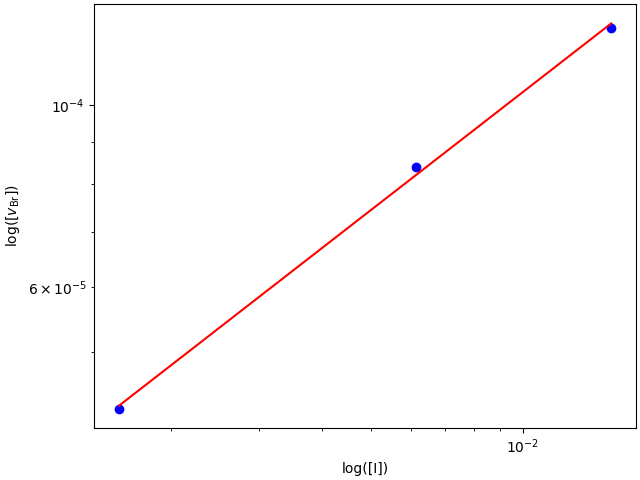
\includegraphics[scale = 0.7]{Bilder/PlotsVersuch1.png}
				\caption{Doppellogarithmische Auftragung der Bruttogeschwindigkeit $v_\text{br}$ auf die Initiatorkonzentration $[I]$.}
				\label{PlotsVersuch1}
			\end{figure}

		Die Fitgerade wird über folgende Gleichung beschrieben:

			\begin{equation}
				\log(v_\text{Br}) = 0.4763 \cdot \log([I]) - 3.0318
			\end{equation}

		Nach Ermitteln der Steigung dieser Gerade konnte die Reaktionsordnung bestimmt werden, welche 0,4763 beträgt.
		Dies ist ziemlich gut, da diese den theoretischen Wert von 0,5 fast erreicht.
		Durch extrapolieren der Fitgerade kann die Geschwindigkeitskonstante $k$ ermittelt werden. 
		Dies wird über folgende Gleichung erreicht:

			\begin{equation}
				k = 10^{-3.0318- \log{[M]}} = 0,000106
			\end{equation}

		
			
		
		

	\subsection{Versuch 2}

		Die Verhältnisse der Integrale der gemessenen NMR-Spektren der Proben sind in Tabelle \ref{Tabelle-Versuch2} gelistet.

		\begin{table}[ht]
			\centering
			\caption{Zusammensetzung und Stoffmengenverhältnisse}
			\label{Tabelle-Versuch2}
			\small % Verringert die Schriftgröße leicht, damit es weniger gedrängt wirkt
			\begin{tabularx}{\textwidth}{@{} c *{8}{X} @{}}
				\toprule
				\textbf{Probe} & \textbf{$m_\text{St}$} & \textbf{$m_\text{MMA}$} & \textbf{$I_\text{St}$} & \textbf{$I_\text{MMA}$} & \textbf{$\frac{m_\text{St}}{m_\text{MMA}}$} & \textbf{$n_\text{St}$} & \textbf{$n_\text{MMA}$} & \textbf{$\frac{n_\text{St}}{n_\text{MMA}}$} \\
				\midrule
				1 & 20,83 & 85,77 & 1,00 & 2,57 & 0,243 & 0,2 & 0,857 & 0,233 \\
				2 & 20,83 & 32,04 & 1,00 & 0,96 & 0,650 & 0,2 & 0,320 & 0,625 \\
				3 & 20,83 & 14,02 & 1,00 & 0,42 & 1,486 & 0,2 & 0,140 & 1,429 \\
				4 & 20,83 & 9,34  & 1,00 & 0,28 & 2,229 & 0,2 & 0,093 & 2,145 \\
				5 & 20,83 & 5,01  & 1,00 & 0,15 & 4,161 & 0,2 & 0,050 & 4,000 \\ 
				\bottomrule
			\end{tabularx}
		\end{table}

		Die Verhältnisse entsprechen dabei den Stoffmengenverhältnissen an Styrol zu MMA in den Polymerketten. Allerdings sind die Integrale noch für unterschiedlich viele 
		Protonen geltend. 
		Für die Umrechnung in ein Massenverhältnis werden die Verhältnisse noch mit dem Signalverhältnis und dem Molekulargewichtsverhältnis von Styrol zu MMA multipliziert. 
		Demnach entspricht das Massenverhältnis der ersten Probe 

		\begin{equation*}
			\frac{m_\text{Styrol}}{m_\text{MMA}} = \frac{1}{2,57} \cdot \frac{\SI{104,15}{\frac{g}{mol}}}{\SI{100,12}{\frac{g}{mol}}} \cdot \frac{3}{5} = 0,243 \text{.}
		\end{equation*}

		Die restlichen Massenverhältnisse der Proben sind in Tabelle \ref{Tabelle-Versuch2} aufgelistet.

	 \subsubsection{Copolymerisationsparameter nach Mayo und Lewis}

		
		Wie in Gleichung \ref{CoPO-r1r2} beschrieben, können die Funktionen für $r_\text{St}$ und $r_\text{MMA}$ bestimmt werden. 
		Daraus Folgen dann folgende Geradengleichungen.

			\begin{eqnarray}
				r_{\text{St},1} =& r_{\text{MMA},1} \cdot 7,167 - 0,139\\
				r_{\text{St},2} =& r_{\text{MMA},2} \cdot 3,07 - 0,161\\
				r_{\text{St},3} =& r_{\text{MMA},3} \cdot 1,754 + 0,447\\
				r_{\text{St},4} =& r_{\text{MMA},4} \cdot 0,658 + 2,263\\
				r_{\text{St},5} =& r_{\text{MMA},5} \cdot 0,196 + 14,547
			\end{eqnarray}

		Diese aufgestellten Geradenfunktionen können graphisch Aufgetragen werden, womit der Graph \ref{VoodooShit} erhalten wird.

			\begin{figure}[H]
				\centering
				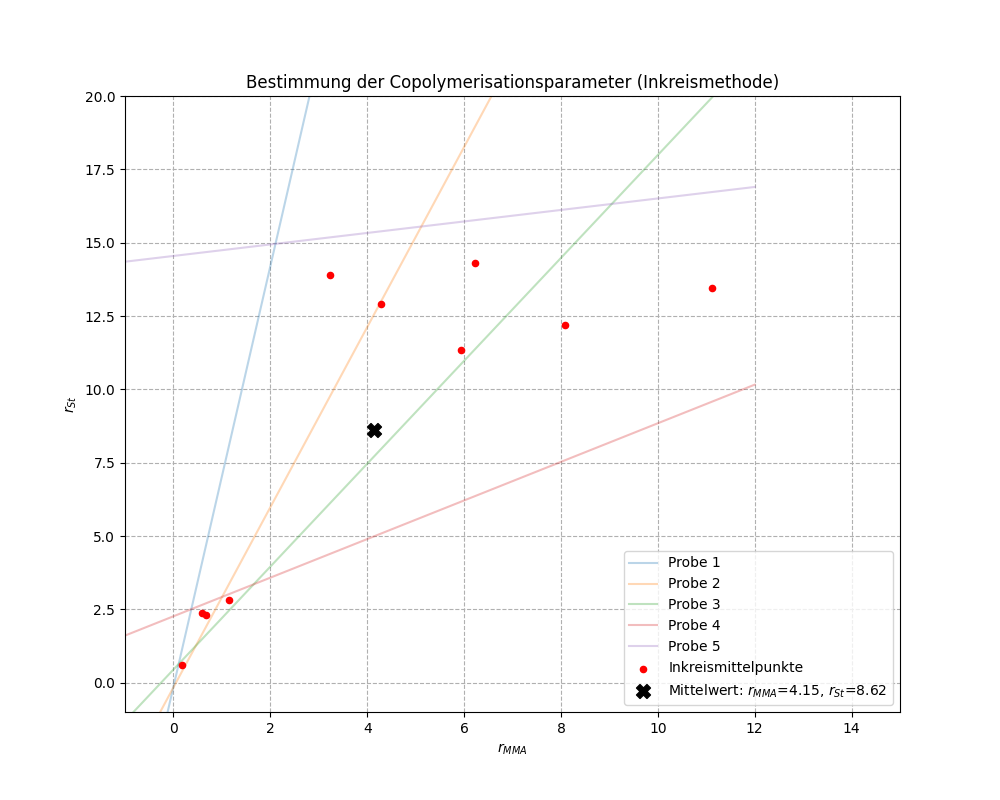
\includegraphics[scale = 0.5]{Bilder/MayoVersuch2.png}
				\caption{Die Abbildung zeigt die graphische Bestimmung der Parameter nach Mayo und Lewis.}
				\label{VoodooShit}
			\end{figure}
			
		Darüber ließen sich die Werte für die jeweiligen Inkreismittelpunkte berechnen.

			\begin{table}[ht]
				\centering
				\caption{Koordinaten der berechneten Inkreismittelpunkte $r_\text{MMA}$ und $r_\text{St}$ .}
				\begin{tabular}{cc}
					\toprule
					\textbf{$r_{MMA}$} & \textbf{$r_{St}$} \\
					\midrule
					0,1771  & 0,6134  \\
					0,5826  & 2,3708  \\
					3,2399  & 13,8874 \\
					0,6784  & 2,3102  \\
					4,2858  & 12,8973 \\
					5,9452  & 11,3267 \\
					1,1504  & 2,8133  \\
					6,2297  & 14,2941 \\
					8,0838  & 12,2002 \\
					11,1200 & 13,4403 \\
					\bottomrule
				\end{tabular}
			\end{table}
		
		Darüber lassen sich nun die Durchschnitte berechnen, welche \O $r_\text{St} = 4.1493$ und \O $r_\text{MMA} = 8,6154$ betragen. 


	\subsubsection{Copolymerisationsparameter nach Fineman und Ross}

		Dabei wird Gleichung \ref{FinemanRoss} mit den Werten aus Tabelle \ref{Tabelle-Versuch2} für jede Rechnung berechnet, wodurch die Punkte erhalten der Geraden erhalten wird. Diese kann dann aufgetragen werden.
		Zusätzlich gilt hier $[M] = n$ da das Volumen konstant ist, daraus folgt als Beispiel für Probe 1.

			\begin{eqnarray}
				\frac{n_\text{St}}{n_\text{MMA}} \cdot \left( 1- \frac{1}{\frac{{m_\text{St}}}{{m_\text{MMA}}}}\right) =& r_1 \cdot \frac{(n_\text{St})^2}{(n_\text{MMA})^2} \cdot \frac{1}{\frac{m_\text{St}}{m_\text{MMA}}} - r_2\\
				\frac{0,0173}{0,0939} \cdot \left( 1 - \frac{1}{0,2429} \right) =& r_1 \cdot \frac{(0,0173)^2}{(0,0939)^2} \cdot \frac{1}{0,2429} - r_2\\
				-0,5739 =& r_1 \cdot 0,1395 -r_2
			\end{eqnarray}
		
		Für die restlichen Proben wurde analog vorgegangen und die Werte sind in Tabelle \ref{Tabelle-Fineman} gelistet.
			
			\begin{table}[h]
				\centering
				\caption{Berechnete Terme für die Linearisierung (Fineman-Ross)}
				\label{Tabelle-Fineman}
				\begin{tabular}{cc}
					\toprule
					$\frac{n_{\text{St}}}{n_{\text{MMA}}} \cdot \left( 1 - \frac{1}{m_{\text{St}}/m_{\text{MMA}}} \right)$ & $\frac{n_{\text{St}}^2}{n_{\text{MMA}}^2} \cdot \frac{1}{m_{\text{St}}/m_{\text{MMA}}}$ \\ 
					\midrule
					-0,728 & 0,224 \\
					-0,336  & 0,601 \\
					0,467  & 1,373 \\
					1,182  & 2,060 \\
					3,039   & 3,845 \\
					\bottomrule
				\end{tabular}
			\end{table}

		Diese Werte werden geplottet und es wird eine Ausgleichsgerade sowie der Achsenabschnitt bestimmt.
		Welche den Werten $r_1$ und $r_2$ entsprechen.

			\begin{figure}[H]
				\centering
				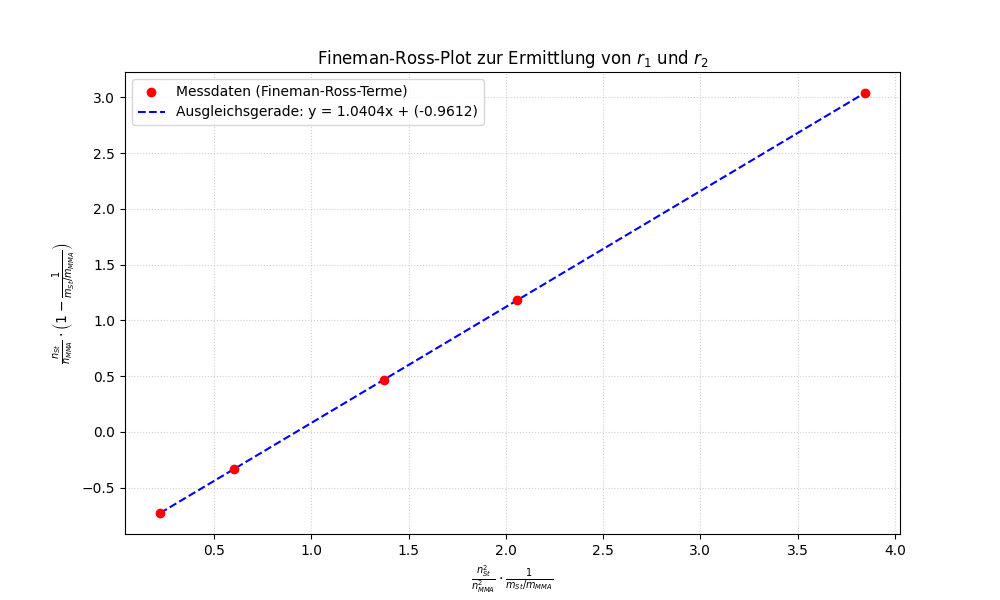
\includegraphics[scale = 0.5]{Bilder/GraphFineman.png}
				\caption{Der Graph zeigt die graphische Bestimmung der Copolymerisationskonstanten über die Fineman-Ross-Methode.}
			\end{figure}

		Daraus ergeben sich die jeweiligen Werte für $r_1 = 1,040$ aus der Steigung und $r_2 = 0,9612$ aus dem Achsenabschnitt.\\

		Beim Vergleich der r-Werte nach Mayo und Lewis mit Fineman und Ross, sind sehr starke Abweichungen zu erkennen. 
		So betragen die r-Werte bei Mayo und Lewis vier- und acht-Mal größer als die nach Fineman und Ross. Abweichungen sind 
		dabei durch die Streuung der Inkreismittelpunkte nach Mayo und Lewis zu erklären, da diese ein Maß dafür ist. Bei 
		Fineman und Ross wird aber eine Gerade gebildet, die durch fünf Datenpunkte verläuft. Die Punkte liegen dabei sehr genau 
		auf der Geraden, weshalb diese Methode deutlich genauere Werte hervorgerufen hat. Gründe für die Ungenauigkeit der 
		Methode nach Mayo und Lewis, beruht womöglich auf einen Fehler der Ansätze oder den relativ feinen Feststoffen die 
		teilweise bei der Fällung isoliert wurden.\\\\

		Abschließend lässt sich das Copolymerisationsdiagramm des Blockcopolymers aus Styrol und MMA erstellen.
		Die Punkte werden über die jeweiligen Gleichungen bestimmt:

			\begin{eqnarray}
				\frac{n_\text{St}}{n_\text{St} + n_\text{MMA}}\\
				\frac{m_\text{St}}{m_\text{St} + \m_\text{MMA}}
			\end{eqnarray}
		
		Dabei wird Gleichung (27) auf Gleichung (28) aufgetragen. Die Ergebnisse der Proben sind in Tabelle \ref{Copolymerisationsdiagramm-Tabelle} gelistet und in Abb. \ref{Copolymerisationsdiagramm-Graph} geplottet.
		
			\begin{table}[h]
				\centering
				\caption{Stoffmengenanteile und Massenanteile der Copolymerisation}
				\label{Copolymerisationsdiagramm-Tabelle}
				\begin{tabular}{cc}
					\toprule
					$\frac{n_{\text{St}}}{n_{\text{St}} + n_{\text{MMA}}}$ & $\frac{m_{\text{St}}}{m_{\text{St}} + m_{\text{MMA}}}$ \\ 
					\midrule
					0,189 & 0,195 \\
					0,385 & 0,394 \\
					0,588 & 0,598 \\
					0,682 & 0,690 \\
					0,800 & 0,806 \\
					\bottomrule
				\end{tabular}
			\end{table}

			\begin{figure}[H]
				\centering
				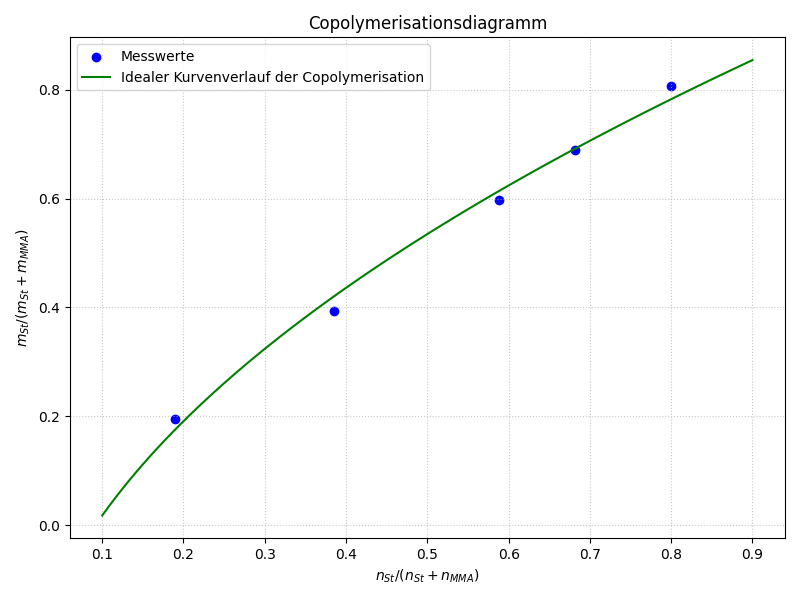
\includegraphics[scale = 0.5]{Bilder/CopoDiagramm.png}
				\caption{Die Abbildung zeigt das Copolymerisationsdiagramm der Copolymerisation von Styrol und MMA}
				\label{Copolymerisationsdiagramm-Graph}
			\end{figure}
		
\section{Fazit}

	

\section{Fragen}

	\subsection{Frage 1}

		\textbf{Während der Versuchsvorbereitung wurden die Ansätze entgast, um
				Sauerstoff aus dem System zu entfernen. Diskutieren Sie kurz die Problematik
				der Anwesenheit von Sauerstoff bei der radikalischen Polymerisation. Könnte
				er auch als Initiator fungieren?}\\
		Es sollte weitestgehend Sauerstofffrei gearbeitet werden, da Sauerstoff als Diradikal vorliegt und ein Kettenabbruch stattfinden kann. 
		Dies gilt auch für die Initiierung der Reaktion. 

		
	\subsection{Frage 2}
		
		\textbf{Was besagen die Begriffe Ceiling- und Floor-Temperatur? Welche
				thermodynamische Gleichung ist dabei relevant?}\\
		Im Allgemeinen beschreibt die ceiling-Temperature die Temperatur einer Reaktion,
		ab welcher eine Depolymerisierung stattfindet. 
		So scheint es als würde keine Reaktion stattfinden.
		Die Floor-Temperatur beschreibt die Temperatur, ab welcher eine Polymerisation begünstigt ist. 
		Sprich ab welcher Temperatur das Gleichgewicht auf die Polymerseite verschoben wird.
		Hierfür spielt die Gibbs-Helmholtz-Gleichung eine große Rolle:

			\begin{equation}
				\Delta G_\text{m} = \Delta H_\text{m} - T \cdot \Delta S_\text{m}
				\label{Gibbs}
			\end{equation}

		
		
	\subsection{Frage 3}

		\textbf{Unter welchen Bedingungen ist die Beziehung $v_w \sim \sqrt{[I]}$ nicht mehr gültig?}\\
		´Siehe Theorie.
		
	\subsection{Frage 4}

		\textbf{Zeichnen Sie den erwarteten Verlauf der Bruttoreaktionsgeschwindigkeit $v_w \sim \sqrt{[I]}$
				in Abhängigkeit des Umsatzes und den entsprechenden Verlauf bei Eintritt des
				Trommsdorff-Effekts (NT-Effekts) auf (s. Kapitel 4.3). Wie ändert sich die
				Abbruchgeschwindigkeit?}\\

		Der Norish-Trommsdorff-Effekt ist in Abbildung \ref{Norish-Trommsdorff} visualisiert.

		\begin{figure}[H]
			\centering
			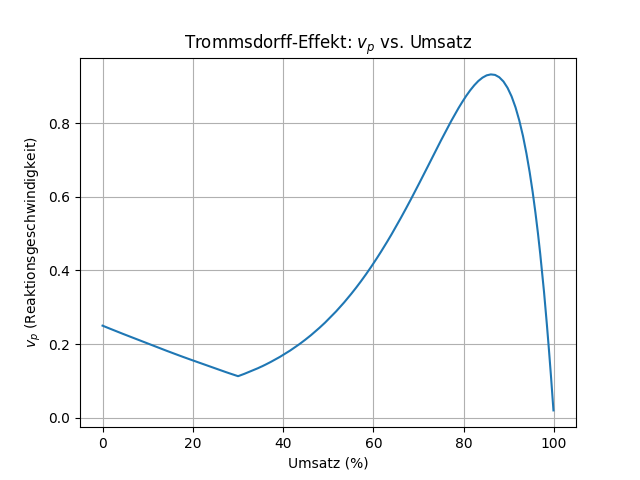
\includegraphics[scale = 0.5]{Bilder/trommsdorff_vd_conv_plot.png}
			\caption{Visualisierung des Norish-Trommsdorff-Effekts.}
			\label{Norish-Trommsdorff}
		\end{figure}
		
		Zu erkennen ist ein plötzlicher Anstieg der Reaktionsgeschwindigkeit. Das liegt daran, dass mit voranschreitendem Umsatz, ebenfalls die 
		Viskosität steigt und dadurch die Ketten sich weniger bewegen. Dadurch können die Radikale der Ketten nur schwer rekombinieren und die 
		Abbruchgeschwindigkeit wird stark herabgesenkt. Da die Monomere allerdings sehr kleine sind, können diese durch die Ketten diffundieren und 
		leicht mit den freien Radikalen polymerisieren.

	\subsection{Frage 5}

		\textbf{Was sind Block- und Pfropfcopolymere? Wie können sie hergestellt werden?
				Gebt je ein Beispiel mit Strukturformal an.\\
				a) $r_1 = 1.00,  r_2 > 1.00$\\
				b) $r_1 = 1.00,  r_2<1.00$\\
				c) $r_1 \rightarrow 0,  r_2 \rightarrow 0$\\
				d) $r_1 \rightarrow \inf,  r_2 \rightarrow \inf$\\
				Unter welchen Bezeichnungen sind die „Grenzfälle“ c) und d) bekannt?}\\

		Ein Blockcopolymer ist, wie der Name schon sagt, ein Blockweise aufgebautes Polymer. Auch zu sehen in Abb. [\ref{Block}].
		Anders als bei dem Blockcopolymer hat das Pfropfcopolymer einen Hauptstrang welcher aus einem Monomer (A) besteht.
		An diesem Hauptstrang sind weitere Polymere (B) quer verbaut.
		Somit gibt es ein Pfropfende und die Querketten [\ref{Propf}]

			\begin{figure}[htbp]
				\centering
				% Erstes Bild
				\begin{subfigure}[b]{0.45\textwidth}
					\centering
					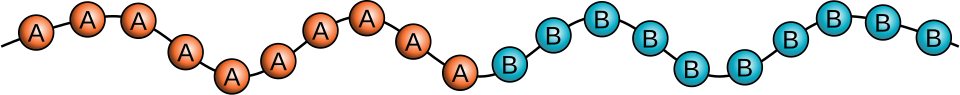
\includegraphics[width=\textwidth]{Bilder/Block_copolymer.png}
					\caption{Abfolge eines Bolckcopolymers. \supercite{noauthor_copolymer_2025}}
					\label{Block}
				\end{subfigure}
				\hfill % Erzeugt flexiblen Zwischenraum
				% Zweites Bild
				\begin{subfigure}[b]{0.45\textwidth}
					\centering
					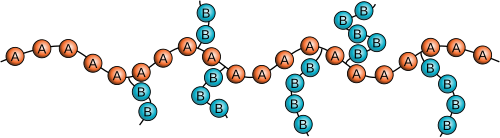
\includegraphics[width=\textwidth]{Bilder/Pfropf.png}
					\caption{Abfolge eines Pfropfcopolymers.\supercite{noauthor_copolymer_2025}}
					\label{Propf}
				\end{subfigure}
				
				\caption{Abfolgen eines Block- sowie Pfropfcopolymers.}
				\label{Block_Pfropf}
			\end{figure}
		
	\subsection{Frage 6}

		\textbf{Welche Konsequenzen haben folgende Copolymerisationsparameter für den
				strukturellen Aufbau von Copolymeren?}\\

		Bei a) wird bevorzugt Monomer B eingebaut und bei b) wird bevorzugt Monomer A eingebaut.
		Bei c) wollen beide Monomere nicht mit sich selbst reagieren somit entsteht ein alternierendes Copolymer.
		Polymer d) ist das gegenteil von Polymer c) sprich die Monomere wollen ausschließlich mit sich selbst reagieren, es wird somit ein
		Blockcopolymer gebildet.
		
	\subsection{Frage 7}

		\textbf{Wie sieht das Copolymerisationsdiagramm für $r_1 > 1$ und $r_2 > 1$ (qualitativ) aus?}\\
	
		Die nachfolgende Abbildung zeigt das Copolymerisationsdiagramm für unterschiedliche Werte, aber auch das für r-Werte von $r_1 = r_2 > 1$.

			\begin{figure}[H]
				\centering
				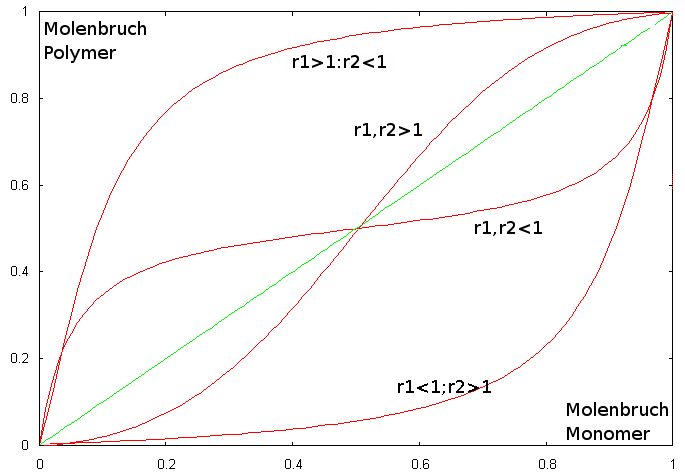
\includegraphics[scale = 0.5]{Bilder/Copolymerisationsdiagramm.png}
				\caption{Verläufe der Copolymerisationskurve für unterschiedliche r-Werte. \supercite{noauthor_copolymerisation_2025}}
				\label{CoPo-Diagramm-Frage}
			\end{figure}

	\subsection{Frage 8}

		\textbf{Welche Methoden für die experimentelle Ermittlung der Zusammensetzung
				von Copolymeren kennen Sie?}\\
		
		Wie bereits oben genannt, können Methoden wie NMR- IR oder UV/Vis-Spektroskopie verwendet werden. 
		Meist werden sich hierbei Eigenschaften des eingebauten Monomers zu Nutze gemacht. 
		
	\subsection{Frage 9}

		\textbf{Was versteht man unter dem „Azeotrop“ im Copolymerisationsdiagramm und
				welchen Werten müssen r1 und r2 genügen, damit ein Azeotrop vorliegen
				kann?}\\
		
		An dem Azeotropen Punkt ist die Copolymerkonzentration dieselbe wie die der Monomerkontzentration.
		Wichtig hierbei ist, dass eine der zwei folgenden Fälle gilt:\\
		Fall 1: $r_1,r_2 < 1$ dabei spricht man von einem stabilen Azeotrop.\\
		Fall 2: $r_1,r_2 > 1$ dabei wird von einem instabielen Azeotrop gesprochen.\\

		Ist lediglich einer der beiden unterschiedlich liegt kein Azeotrop vor.
		
	\subsection{Frage 10}

		\textbf{Bestehen strukturelle Unterschiede zwischen Polymeren aus radikalisch bzw.
				anionisch initiierten Copolymerisationen (bei gleichen Werten für r1 und r2)?}\\
		
		Es bestehen kein Struktureller unterschied in der groben Backbone Struktur. Ein großer Unterschied liegt in der Verzweigtheit. 
		Bei der radikalischen Polymerisation können kettenübertragungen stattfinden wodurch eine Verzweigung entsteht.
		Bei der ionischen ist dies nicht möglich, dementsprechend entsteht ein lineares Polymer.
		Unteranderem liegt ein Unterschied in der Dispersität vor. Da bei der radikalischen Polymerisation die Ketten alle unterschiedlich lang sind.
		Bei der ionischen hingegen sind die Ketten alle gleich lang da alle gleichzeitig initiiert werden.
		
	\subsection{Frage 11}

		\textbf{Warum erhält man im 1H-NMR-Spektrum für die Methoxygruppe im
				Copolymer, im Gegensatz zum MMA-Monomer, nicht nur ein Signal?}\\
		
		Der Grund für unterschiedliche Verschiebungen liegt in der Umgebung der Methoxygruppe.
		Da das MMA-Moynomer zufällig in die Kette eingebaut wird und dementsprechend unterschiedliche Umgebungen aufweist.
		Daraus folgen unterschiedliche Signale welche an unterschiedlichen Verschiebungen zu sehen sind.

	\subsection{Frage 12}

		\textbf{Ermitteln Sie die mittlere Sequenzlänge und die Blockzahl für die
				Monomerpaare Styrol und Vinylidenchlorid (r1 = 2.0, r2 = 0.14). Die Monomerkonzentrationen betragen 25 mol-% Styrol und 75 mol-%
				Vinylidenchlorid. Erläutern Sie bitte kurz das Ergebnis. (mit Rechenweg)}\\
		
		Die mittlere Sequenzlänge kann über folgende Gleichung berechnet werden.	
			
			\begin{equation}
				\bar{I_\text{St}} = r_1 \cdot \frac{[M_1]}{[M_2]} + 1
			\end{equation}
				
		Durch einsetzten beider Werte ergibt sich dabei für Styrol ein Wert von $\bar{I_\text{St}} = 1,67$ 
		und für Vinylidenchlorid ein Wert von $\bar{I_\text{VC}} = 1,42$
		Daraus lässt sich sagen, dass die Blöcke im Durchschnitt aus 1,67 Einheiten bestehen.
		Die Blockzahl wird anschließend nach folgender Gleichung berechnet:
		
			 \begin{equation}
				R = \frac{200}{2 + r_1 \frac{[M_1]}{M_2} + r_2 \frac{[M2]}{[M_1]}} + 1
			 \end{equation}
		
		Dies Resultiert in diesem Fall in einer Blockzahl von $R = 64,8$. Dies bedeutet, dass es in 100 Einheiten 64,8 Blöcke sind.
\printbibliography

\end{document}